
\subsubsection{Modifying the dataset for the neural network}\label{dataset-creation}

Once the dataset to be achieved has been explained along with the motivation, this section will explain the steps followed to achieve this result. The dataset at this point has as many rows as there have been trips between 2014 and 2019. For each row, there are two attributes: \small{\verb|from_station_id|} \normalsize  and \small{\verb|start_time|} \normalsize .
\newline


In this module we want to modify this dataset to obtain another one containing the vectors that can be used as input vectors in the network. That is, we want to create a dataset that contains in each row the intervals and in each column the data of that interval: hour, \small{\verb|day_of_week|} \normalsize , \small{\verb|month|} \normalsize  and \small{\verb|quantity_j|} \normalsize . When all the steps of this module have been completed, the data will be saved in a file called \small{\verb|intervals.csv|} \normalsize  and a sample of this data can be seen in Appendix \ref{app:intervals_dataset}.
\newline

First, the code of this module, loads the data of the previous module from the \acrshort{csv} \small{\verb|trips.csv|} \normalsize  file:
\begin{minted}[fontsize=\footnotesize]{python}
import pandas as pd

# Read CSV as DataFrame an use datetime as index
df = pd.read_csv("/path/to/trips.csv", index="start_time")
\end{minted}


Once the \small{\verb|DataFrame|} \normalsize  has been loaded, the following steps have been carried out:
\begin{enumerate}
    \item \underline{Grouping interval trips}: This step aims to group the trips that start at each of the stations into intervals. Different sizes of intervals have been studied, such as $15$ or $30$ minute intervals, but finally, 1 hour has been chosen because the number of rows is considerably reduced and it is still a valid interval and not very wide. 
    \newline
    
    The different trips have been grouped in intervals according to the \small{\verb|from_station_id|} \normalsize  and \small{\verb|start_time|} \normalsize  columns. As an example, suppose you have the following \small{\verb|DataFrame|} \normalsize  in the \small{\verb|df|} \normalsize  variable:

    \begin{table}[H]
    \footnotesize
    \centering
    \begin{tabular}{c|rr}
        \toprule
          \textit{start\_time} & \textit{from\_station\_id}  \\
        \midrule
        
        10:10 - 12/2/2018 & 48\\
        10:28 - 12/2/2018 & 15\\
        10:56 - 12/2/2018 & 15\\
        11:03 - 15/2/2018 & 15\\
        11:12 - 15/2/2018 & 48\\
        11:15 - 15/2/2018 & 15\\
        11:18 - 15/2/2018 & 15\\
        11:31 - 15/2/2018 & 15\\
        11:44 - 15/2/2018 & 48\\
        11:49 - 15/2/2018 & 15\\
        22:00 - 16/2/2018 & 15\\
        22:15 - 16/2/2018 & 48\\
        22:37 - 16/2/2018 & 193\\
        22:56 - 16/2/2018 & 48\\
        \bottomrule
        
    \end{tabular}
    \cprotect\caption{Example of dataset stored in \small{\verb|trips.csv|} \normalsize }
    \label{tab:starttime_withsid}
    \end{table}
    
    The code used to group the trips by intervals and by station has been the following:
    
    \begin{minted}[fontsize=\footnotesize]{python}
INTERVAL = "1H"  # It could be also 15Min

df = df.groupby('from_station_id') \
      .resample(INTERVAL, on='start_time') \
      .size() \    # Resampling using the sum rule
      .to_frame()  # Converts it to DataFrame
    \end{minted}
    
After executing these lines of code and using the example in table \ref{tab:starttime_withsid} you can see that the result is as follows:
    \begin{table}[H]
    \footnotesize
    \centering
    \begin{tabular}{c|rr}
        \toprule
          \textit{start\_time} & \textit{from\_station\_id} & \textit{quantity}  \\
        \midrule
        
        10:00 - 12/2/2018 & 15 & 2\\
        10:00 - 12/2/2018 & 48 & 1\\
        10:00 - 12/2/2018 & 193 & 0\\
        11:00 - 15/2/2018 & 15 & 5\\
        11:00 - 15/2/2018 & 48 & 2\\
        11:00 - 15/2/2018 & 193 & 0\\
        22:00 - 16/2/2018 & 15 & 1\\
        22:00 - 16/2/2018 & 48 & 2\\
        22:00 - 16/2/2018 & 193 & 1\\
        \bottomrule
    \end{tabular}
    \cprotect\caption{Example of the dataset grouped by season and by interval.}
    \label{tab:justintervals}
    \end{table}
    
    
    \item \underline{Pivot by intervals}: This step aims to group all the intervals into one alone, thus increasing the number of columns and reducing the number of rows. In other words, you want each row to represent an interval and each column to represent a season. Using the same example as in the previous step, the final \small{\verb|DataFrame|} \normalsize  would look like this.
    \begin{table}[H]
    \footnotesize
    \centering
    \begin{tabular}{c|rrr}
        \toprule
        \textit{start\_time} & \textit{quantity\_15} & \textit{quantity\_48} & \textit{quantity\_193}  \\
        \midrule
        10:00 - 12/2/2018 & 2 & 1 & 0 \\
        11:00 - 15/2/2018 & 5 & 2 & 0 \\
        22:00 - 16/2/2018 & 1 & 2 & 1 \\
        
        \bottomrule
    \end{tabular}
    \cprotect\caption{Example of a dataset containing the intervals.}
    \label{tab:intervals_example}
    \end{table}
    
    Primarily, the code used for this step makes use of the \small{\verb|pivot()|} \normalsize  pandas function:
    \begin{minted}[fontsize=\footnotesize]{python}
# Prepare the new columns names for each station
df["quantity_index"] = "quantity_" + \
                        df["from_station_id"].astype("str")

# We don't need from_station_id anymore
df = df.drop(columns=["from_station_id"])

# Make the pivot around quantity_index column and
# set the value of the column the same value as
# quantity from before saving quantity from
df = df.pivot(columns='quantity_index', values='quantity')

# If station any interval didn't have any trips for
# a station, then fill it with 0
return df.fillna(0)
    \end{minted}
    
    If you compare table \ref{tab:starttime_withsid} with table \ref{tab:intervals_example} you can see that the amount of data has been reduced considerably and only the necessary information that the network will need has been selected.
    \newline
    
    \item \underline{Get the time variable}: The \small{\verb|start_time|} \normalsize  column is a Series with timestamps and therefore has more information than necessary (year, month, day, hour, minute, second...). The only temporary information needed is a subset of these values. Specifically, the values that have been thought to be useful are: the time, the day of the week (it is not the same on a Monday as on a Saturday) and the month (it is not the same on a winter month as on a summer month). These are the simplest values that have been used, but this does not mean that other data that provide more information can't be used, such as: day of the month, year or the minute. 
    \newline
    
  Using the variables in this way and not using the timestamp directly to the network, the model can learn patterns based on simpler variables such as the time, day of the week or month, and not with a 64-bit number that barely provides any information since the network would take them as ascending values without any criteria.
    
  The following lines of code have been used to create the new columns with the attributes explained above:
    \begin{minted}[fontsize=\footnotesize]{python}
# Index and start_time column is the same

df['hour'] = df.index.hour              # Number between 0-23
df['day_of_week'] = df.index.dayofweek  # Number between 0-6
df['month'] = df.index.month            # Number between 1-12
    \end{minted}
    
    At the end of this step there will therefore be the following columns for each of the intervals: \small{\verb|start_time|} \normalsize , \small{\verb|hour|} \normalsize , \small{\verb|day_of_week|} \normalsize , \small{\verb|month|} \normalsize  and one column for each station. The column \small{\verb|start_time|} \normalsize  is not deleted because it is the column used as an index and helps to understand the information you are working with. But it will not be used by the neural network.
    \newline
    
    Using the same example as the previous steps, the table would look like this:
    \begin{table}[H]
    \footnotesize
    \centering
    \begin{tabular}{c|rrr|rrr}
        \toprule
        \textit{start\_time} & \textit{quantity\_15} & \textit{quantity\_48} & \textit{quantity\_193} & \textit{hour} & \textit{day\_of\_week} & \textit{month} \\
        \midrule
        10:00 - 12/2/2018 & 2 & 1 & 0 & 10 & 0 & 2 \\
        11:00 - 15/2/2018 & 5 & 2 & 0 & 11 & 3 & 2 \\
        22:00 - 16/2/2018 & 1 & 2 & 1 & 22 & 4 & 2 \\
        
        \bottomrule
    \end{tabular}
    \cprotect\caption{Example of a final dataset to be used by the neural network.}
    \label{tab:intervals_example}
    \end{table}
    
    
    At this point, the possibility of storing the information of the temporal variables in the form of a signal with values between the ranges $[-1, 1]$ using sine and cosine \cite{reddit_time} was also studied. This allows the model to have access to the temporal information with continuous and not discrete values as it can be seen in figure \ref{fig:hour-stepvssignal} below. The results obtained with both techniques were similar, so for simplicity we leave it with discrete values.
    
  \begin{figure}[H]
  \centering
  \subfloat[Time with continuous values from $-1$ to $1$]{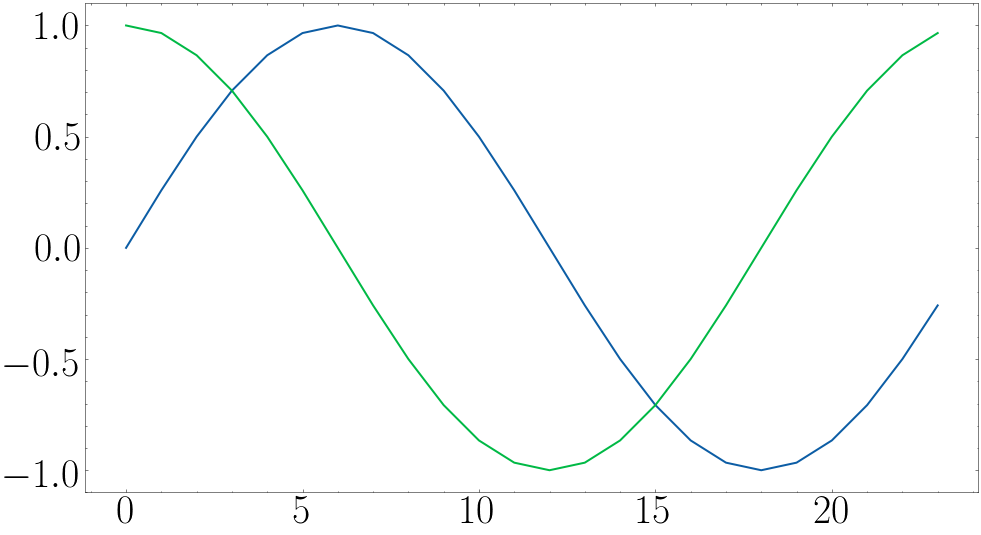
\includegraphics[width=0.4\textwidth]{images/solution/modules/hour_signal.png}\label{fig:f1}}
  \hfill
  \subfloat[Time with discrete values from $0$ to $23$]{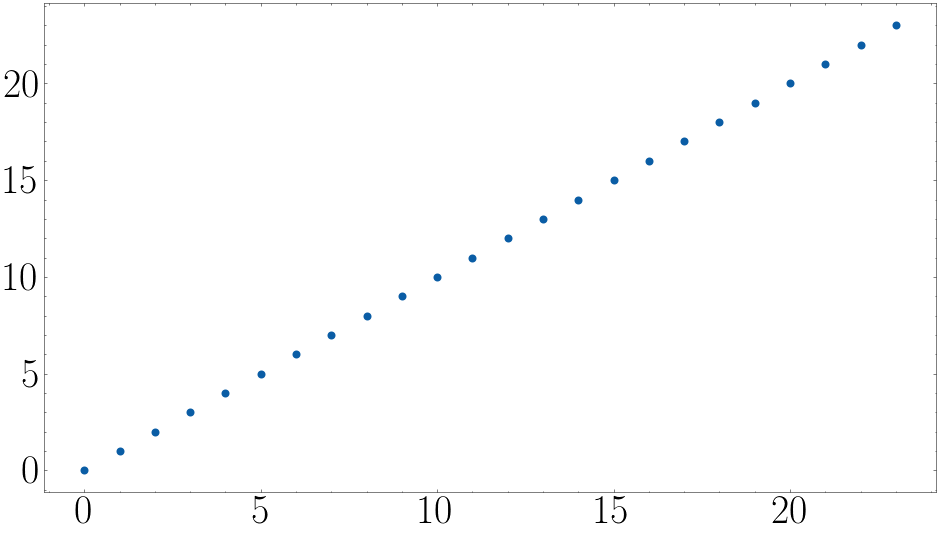
\includegraphics[width=0.4\textwidth]{images/solution/modules/hour_steps.png}\label{fig:f2}}
  \caption{Possible ways of representing the hour variable.}
  \label{fig:hour-stepvssignal}
\end{figure}
    
\end{enumerate}

The \small{\verb|DataFrame|} \normalsize  obtained by this module is saved in a \acrshort{csv} file called \small{\verb|intervals.csv|} \normalsize  which will be used by the following modules whose content will have a similar structure to that shown in table \ref{tab:intervals_example}.

\begin{minted}[fontsize=\footnotesize]{python}
# Save df in a CSV file
df.to_csv("path/to/intervals.csv")
\end{minted}